\documentclass{article}
\usepackage{amsmath,amsfonts,amsthm,amssymb,mdframed}
\usepackage{geometry, enumitem,url, kotex}
\usepackage{setspace,graphicx}

\geometry{a4paper, margin=2cm}

\title{An Example with Two Lagrange Multiplier}
\author{}
\date{\today}

\begin{document}
\setstretch{1.5}
\maketitle

\begin{center}
Maximize $f(x,y,z)$ subject to \(\begin{cases}g(x,y,z)=c\\h(x,y,z)=k\end{cases}\)
\end{center}

\tableofcontents

\newpage

%%
\section{라그랑지 승수법 (두 개의 제약조건)}
만약 $f$가 $(x_0, y_0, z_0)$에서 최솟값을 가지면

\[
\begin{cases}
\nabla f+\lambda\nabla g+\mu\nabla h=0\\
g=0\\
h=0
\end{cases}
\text{ at }(x_0,y_0,z_0)
\]

을 만족시킨다. (단, $\lambda$, $\mu$는 실수)

다시 말해

\[
\begin{cases}
\nabla f(x_0,y_0,z_0)+\lambda\nabla g(x_0,y_0,z_0)+\mu\nabla h(x_0,y_0,z_0)=0\\
g(x_0,y_0,z_0)=0\\
h(x_0,y_0,z_0)=0
\end{cases}
\]

이다.
더 자세히 쓰면

\[
\begin{cases}
f_x(x_0,y_0,z_0)+\lambda g_x(x_0,y_0,z_0)+\mu h_x(x_0,y_0,z_0)=0\\
f_y(x_0,y_0,z_0)+\lambda g_y(x_0,y_0,z_0)+\mu h_y(x_0,y_0,z_0)=0\\
f_z(x_0,y_0,z_0)+\lambda g_z(x_0,y_0,z_0)+\mu h_z(x_0,y_0,z_0)=0\\
g(x_0,y_0,z_0)=0\\
h(x_0,y_0,z_0)=0
\end{cases}
\]
이다.
(단, $f_x=\frac{\partial f}{\partial x}$, $f_y=\frac{\partial f}{\partial y}$, $f_z=\frac{\partial f}{\partial z}$)

\begin{center}
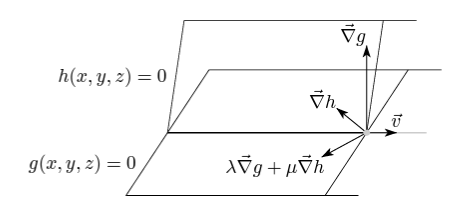
\includegraphics[width=.6\textwidth]{figure.png}
\end{center}

\newpage
%%
\section{설명}
두 조건 $g(x,y,z)=0$, $h(x,y,z)=0$ 하에서 $f$가 최솟값을 가진다고 가정하자.
곡면 $g(x,y,z)=0$과 곡면 $h(x,y,z)=0$은 (대부분의 상황에서) 교선 $g=h=0$을 가진다.
$P$는 이 교선 위에 위치한다.

이때 교선 $g=h=0$은 (일반적으로) 곡선인데, 이 곡선 위의 점 $P$에서의 한 접벡터(tangent vector)를 $v$라고 하자.
$f$가 교선 $g=h=0$ 상에서의 최댓값을 점 $P$에서 가지므로, $f$의 $P$에서의 $v$방향의 방향도함수(directional derivative)는 0보다 크거나 같다 ; 
\[
D_vf(x_0,y_0,z_0)\ge0,\quad \nabla f(x_0,y_0,z_0)\cdot v\ge0\tag{$*$}
\]
마찬가지의 이유로, $f$의 $P$에서의 $-v$방향의 방향도함수도 0보다 크거나 같다 ; 
\[
D_{-v}f(x_0,y_0,z_0)\ge0,\quad\nabla f(x_0,y_0,z_0)\cdot(-v)\ge0,\quad
\nabla f(x_0,y_0,z_0)\cdot v\le0\tag{$**$}
\]
$(*)$, $(**)$로부터
\[
\nabla f(x_0,y_0,z_0)\cdot v=0\tag{$1$}
\]
이다.

한편, 벡터 $v$는 곡면 $g(x,y,z)=0$에 속하므로,\\
벡터 $v$는 곡면 $g(x,y,z)=0$의 $P(x_0,y_0,z_0)$에서의 접평면에 속하고,\\
벡터 $v$는 곡면 $g(x,y,z)=0$의 $P(x_0,y_0,z_0)$에서의 접평면의 법선벡터$\left(=\nabla g(x_0,y_0,z_0)\right)$와 직교한다;
$$v\perp \nabla g(x_0,y_0,z_0)$$
\[\nabla g(x_0,y_0,z_0)\cdot v = 0\tag{2}\]
이다.
마찬가지로,
\[\nabla h(x_0,y_0,z_0)\cdot v = 0\tag{3}\]
이다.

대부분의 상황에서는 $g(x_0,y_0,z_0)$와 $h(x_0,y_0,z_0)$가 평행하지 않다.
즉, 두 벡터가 평행하지 않는 상황만을 가정하자.
그러면 (1), (2), (3)으로부터 $\nabla f(x_0,y_0,z_0)$는 $\nabla g(x_0,y_0,z_0)$와 $\nabla h(x_0,y_0,z_0)$의 일차결합이다.
즉
$$\nabla f(x_0,y_0,z_0)=(-\lambda)\nabla g(x_0,y_0,z_0)+(-\mu)\nabla h(x_0,y_0,z_0)$$
인 실수 $\lambda$, $\mu$가 존재한다.

따라서
$$\nabla f(x_0,y_0,z_0)+\lambda\nabla g(x_0,y_0,z_0)+\mu\nabla h(x_0,y_0,z_0)=0$$
이 성립한다.
한편, $g(x_0,y_0,z_0)=0$, $h(x_0,y_0,z_0)=0$이 성립하는 것은 당연하므로, \textbf{1}에서 말한 라그랑지 승수법이 성립한다.


%%
\section*{원 글 출처}
\url{https://personal.math.ubc.ca/~feldman/m226/multiLagrange.pdf}


\end{document}